\chapter{Data Aggregation With Internal Verification} % (folit
\label{cha:Data Aggregation With Internal Verification}

% \section{System Design importantplementations}
	The high level idea of the aggregate commit with verification scheme is that all the sensor nodes in the network send the signature of the message along with the message.
	They send their certificates if the parent node does not have it already.
	The parent node verifies all the received signatures from its children.
	And proceeds with the aggregation process.
	After aggregation, the parent node can throw away all the signatures from its children and signs the message of its children or it can pass its children's signatures to its parent. 
	The pros and cons of each approach are discussed in the following sections. 
	And once the base station receives the aggregated value it starts the verification process. 
	If there is no malicious activity in the network then  it accepts the result and takes an action.
	If the malicious activity is detected during the verification phase then the base station starts interactive activity to detect an adversary. 

\section{Data-Item}
	
	We describe structure of the data-item and its signature, used in creating the commitment tree for the aggregate commit with verification approach. And differences between the data-item and the label structure of SHIA, with rational behind it.
	\begin{definition}
		\label{def:data-item}
		A commitment tree is a binary tree where each vertex has an associated data-item representing the data that is passed on to its parent. The data-items have the following format:

		$\hspace{100pt}$ \textbf{$<\ $id, count, value, commitment$\ >$}\\
	Where $id$ is the unique ID of the node; $count$ is the number of leaf vertices in the subtree rooted at this vertex; $value$ is the SUM aggregate computed over all the leaves in the subtree and $commitment$ is a cryptographic commitment.
	\end{definition}
	Each sensor node creates its own data-item during commitment tree generation process which is called the leaf vertex of the node.
	For example, sensor node $S$ creates its data-item $S_{0}$ as follows:
	\begin{equation}
		\label{eq:data-item}
	 	S_{0} =\ <S_{id}, 1, S_{value}, H(N||1||S_{value})>
	 \end{equation}
	where $S_{id}, S_{value}$ is the unique ID and sensor reading of the sensor node $S$. 
	The count is $1$ as there is only vertex in the subtree rooted at $S$, $H$ is the collision resistant hash function, and $N$ is the query nonce.

	The first difference between SHIA's label structure and our data-item structure is that we remove the $complement$ field from the label structure Defined \ref{def:label}. 
	We think the complement filed is redundant information in the label. 
	The complement field is used by the base station (the querier, according to SHIA), before the result checking phase, to verify \textbf{SUM + COMPLEMENT =} $\textbf{n} \cdot \textbf{r}$ ; where $\textbf{n}$ is the number of nodes in the network, $\textbf{r}$ is the upper bound on the allowed sensor readings.
	We can achieve the same upper bound without the complement field.
	As the querier knows $n, r$ and it gets SUM from the root of the aggregation tree.
	If \textbf{SUM} $> \textbf{n} \cdot \textbf{r}$ , then the base station knows some node or nodes in the network reported out of range readings.

	The second difference between SHIA's label structure and our data-item structure is that we include unique ID of the node in its data-item.
	SHIA does not have the ID field in their label structure as they do not do internal verification while creating a commitment tree and while distributing off-path values.
	Also, in the label format ID of the node is hashed in the commitment field after the first aggregation and virtually gets lost.
	Hence, SHIA can not provide security services such as authenticity, non-repudiation and is vulnerable to all sorts of active attacks.
	We do internal verification while creating the commitment tree and distributing off-path values.
	So, it is necessary for any aggregate node to know the ID of all the received data-items in its forest, for the verification of the received signatures as shown in the following sections.

	\subsection{Signing and Verification of the Data-Item}
		\label{subsection:Signing and Verification of the Data-Item}
		Each sensor node sends the signature of its data-item signed by itself using its own secret key. 
		For example, the signature of $S_{0}$ of the Equation \ref{eq:data-item} is given as follows:
		\begin{equation}
			\textsf{S} = \textsf{Sign}_{S_{S}}(S_{0})
		\end{equation}
		where $S_{S}$ is the secret key of the sensor node $S$, $\textsf{Sign}$ is the signing algorithm.
		The parent node receives the data-item and its signature from its child. 
		It also receives the certificate from its child which is shown in Table \ref{table:digital-certificate}.
		\begin{table}[!htb]	
			\begin{center}
				\begin{tabular}{ |l| }
			    \hline
			    Unique ID of the sensor node \\
			    \hline
			    Public key of the sensor node \\	
			    \hline
			    Certification Authority's name \\
			    \hline
			    Certification Authority's digital signature \\
			    \hline
				\end{tabular}
			\end{center}
	  	\caption{Digital Certificate}
		  \label{table:digital-certificate}
	  \end{table}
	  From the digital certificate the parent node receives the public-key of its child, which is necessary to verify the signature.
	  For example, the parent node of $S$ verifies $\textsf{Sign}_{S_{S}}(S_{0})$ as follows:
	  \begin{equation}
			\textsf{Verify}_{P_{S}}(S_{0},\textsf{S}) = 
			\begin{cases}
			 \textbf{true}\ \mbox{with probability of 1} & if\ \textsf{S} = \textsf{Sign}_{S_{S}}(S_{0})\\
			 \textbf{false}\ \mbox{with overwhelming probability} & if\ \textsf{S} \neq \textsf{Sign}_{S_{S}}(S_{0})
			\end{cases}
			\label{eq:verification}
		\end{equation}
	  where $P_{S}$ is the public key of $S$, $\textsf{Verify}$ is the verification algorithm.
	
	\subsection{Security Benefits}
		\label{subsec:security benefits of signing the data-item}
		% \textcolor{red}{remove payload}
		While creating the commitment tree, the sensor $S$ sends the data-item $S_{0}$, and its signature $\textsf{S}$ to its parent in the aggregation tree.
		The signature allows the parent node to verify the \textit{authenticity} of the sensor node.
		As only sensor node $S$ can create the signature using its secret key. 
		The signature $\textsf{S}$ assures the \textit{integrity} of the data-item $S_{0}$.
		Because either the data-item or the signature has been tampered in any way the verification algorithm return false.
		Furthermore, it allows the sender to have the proof for the sent data-item.
		And the receiver for the proof for the received data-item, providing the security service of \textit{non-repudiation}.
		The digital signature depends on the message so the parent node can not reuse the signature for other data-items in the future.
		Hence, protecting the network against the \textit{replay attacks}.
		Hence, it protects against the \textit{active attacks}.

\section{Commitment Payload}

	We define commitment payload based on the commitment forest Defined in \ref{def:commitment-forest}.
	\begin{definition}
		A \textbf{commitment payload} is the concatenation of a set of data-items of the root vertices of the trees in the outgoing commitment forest.
	\end{definition}
	% We use the term payload for commitment payload and the term forest for the commitment forest.
	For brevity, we use the term forest, payload instead of commitment forest, commitment payload respectively.
	Consider, the aggregation tree shown in Figure \ref{fig:Palm aggregation tree}, where $B$ is the parent of $A$, $C$ is the parent of $B$ and $D$ is the parent of $C$. 
	\begin{figure}[h!]
		\centering
		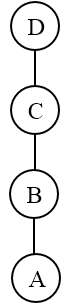
\includegraphics[scale = 1]{images/palm-aggregation-tree.png}
		\caption{Palm Shaped Aggregation Tree}
		\label{fig:Palm aggregation tree}
	\end{figure}
	While creating the commitment tree $A$ creates its data-item $A_{0}$ according to Equation \ref{eq:data-item}.
	$A$ sends only one data-item to $B$ therefore $A$'s payload with its signature is given as follows:
	\begin{equation}
		A_{p} =\ <A_{0}>\ ;\ \textsf{Sign}_{S_{A}}(A_{p})
	\end{equation}
	The sensor node $C$'s payload is shown in Figure \ref{fig:Commitment payload of C}.
	The commitment tree generation process is described in the later sections. 
	The sensor node $C$ sends two data-items to $D$ therefore $C$'s payload with its signature is given as follows:
	\begin{equation}
	 	C_{p} =\ <B_{1}\ ||\ C_{0}>\ ;\ \textsf{Sign}_{S_{C}}(C_{p})
	\end{equation}
	\begin{figure}[h!]
		\centering
		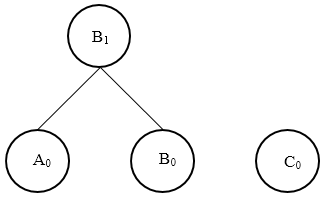
\includegraphics[scale = 1]{images/commitment-payload-of-C.png}
		\caption{Commitment Payload of Sensor Node $C$}
		\label{fig:Commitment payload of C}
	\end{figure}
	The verification of the received signatures of the payload is done by the parent node in the same way described in Section \ref{subsection:Signing and Verification of the Data-Item}.

	\subsection{Security Benefits}
		In similar way, the signature $\textsf{Sign}_{S_{S}}(S_{p})$ assures the integrity and authentication of the payload $S_{p}$.
		It is like the signature for the transmission.
		To the sender, it assures that all the data-items in the payload were successfully transmitted.
		To the receiver, it assures that all the data-items were received successfully.

		In addition to all the security benefits mentioned in Subsection \ref{subsec:security benefits of signing the data-item}, signature on the $C$'s payload $\textsf{Sign}_{S_{C}}(C_{p})$ assures that the sensor node $C$ sent only two data-items $C_{0},B_{1}$ in its payload.
		And none of the data-items in its payload have been left stranded.
		It is true for the sensor node $A$.
		It like the signature for the transmission.

\section{Differences from SHIA}

	The key difference between the SHIA's approach and our approach is that, in addition to sending the data-item, each sensor node sends the signature of the data-item and the signature of its payload to its parent.
	It sends its certificate as well if the parent node does not have it in its memory already.
	The parent node gets its child's public key from its certificate, which is used in verifying the signature. 
	The certificate is issued by the base station which is a trusted third party in our design.
	The parent node verifies all the received signature using its children node's public key.
	Details of the signing and verification processes are shown in Figure \ref{fig:digita-signature}.
	Only, after doing the verification the parent node proceeds to the aggregation and creating the commitment tree.
	
	\subsection{Bandwidth Analysis}

	Cite resources for this.
	\cite{ecdsa2009186}
	Typical size of the data-item packet is $400$ bits.
	If one uses Elliptic Curve Digital Signature Algorithm (ECDSA) then the size of signature is $500$ bits.
	And the certificate size is $1500$ bits.
	So, at max we have to send additional $2000$ bits with the data-item.
	We think it is worthwhile to send these additional bits.
	Because of all the security benefits we gain from it. 
	\textbf{Note:} The packets size are close approximate to the actual packet size. 
	The actual packet size may differ based on the implementation.

\section{Two ways of Forwarding the Commitment Payload}	
	
	In the previous section, we described the signing process where a sensor node has a single data-item in its payload.
	Here, we describe the signing process where an aggregate node has more than one data-item in its payload.
	% The signature on the payload assures that an aggregate node sent only the data-items included in the payload signature.
	% It assures the authenticity, non-repudiation, integrity of all the data-items included in the payload.
	For example, the aggregation tree shown in Figure \ref{fig:Palm aggregation tree}, the payload of sensor node $C$ is show in Figure \ref{fig:Commitment payload of C}.

	The sensor node $C$ sends all the data-items in its payload with their respective signatures to its parent sensor node $D$.
	Furthermore, $C$ sends the signature of its payload $\textsf{Sign}_{S_{C}}(C_{0}||B_{1})$ to $D$.

	\begin{equation}	
		\begin{array}{l}
			C_{0} =\ <C_{id}, 1, C_{value}, H(N||1||C_{value})>;\ \textsf{Sign}_{S_{C}}(C_{0})\\
			B_{1} =\ <B_{id}, 2, B_{1value}, H(N||2||B_{1value}||A_{0}||B_{0})>;\ \textsf{Sign}_{S_{B}}(B_{1})\\
			C_{p} =\ <C_{0}||B_{1}>;\ \textsf{Sign}_{S_{C}}(C_{p})
		\end{array}
		\label{eq:forwarding-payload-without-resigning}
	\end{equation}

	% This example showcases another important aspect of the protocol.
	% It shows two different ways of creating a commitment tree.
	The sensor node $C$ has two data-items $C_{0},B_{1}$ in its payload as shown in Equation \ref{eq:forwarding-payload-without-resigning}. 
	It sends the $\textsf{Sign}_{S_{B}}(B_{1})$, $\textsf{Sign}_{S_{C}}(C_{0}) $ and $\textsf{Sign}_{S_{C}}(C_{p})$ where $C_{p} = < C_{0}||B_{1} >$ to its parent node $D$.
	It requires the parent node $D$ to know the public key of the sensor nodes $C$ and $D$, hence their certificates.
	Instead of that the sensor node $C$ can verify the $\textsf{Sign}_{S_{B}}(B_{1})$ then remove the old signature and create new signature $\textsf{Sign}_{S_{C}}(B_{1})$ signed by itself on the data-item $B_{1}$ as follows:
	\begin{equation}	
		\begin{array}{l}
			B_{1} =\ <B_{id}, 2, B_{1value}, H(N||2||B_{1value}||A_{0}||B_{0})>;\  \textcolor{red}{\textsf{Sign}_{S_{C}}(B_{1})}\\
			C_{0} =\ <C_{id}, 1, C_{value}, H(N||1||C_{value})>;\ \textsf{Sign}_{S_{C}}(C_{0})\\
			C_{p} =\ <C_{0}||B_{1}>;\ \textsf{Sign}_{S_{C}}(C_{p})
		\end{array}
		\label{eq:forwarding-payload-with-resigning}
	\end{equation}
	In this case, the parent node $D$ needs to know the public key of only the sensor node $C$ as it receives all the signatures signed by the sensor node $C$. 
	Therefore, $D$ need to know only the certificate of $C$.
	The Equation \ref{eq:forwarding-payload-without-resigning}, \ref{eq:forwarding-payload-with-resigning} represents two different ways of designing the protocol.
	To give an analogy with the real world application consider the following example.
	One want to buy a diamond from the local diamond retailer.
	Diamond is an expensive commodity so the end customer wants to verify its authenticity and integrity before purchasing.
	Suppose, the diamond was created by the manufacturer in Africa, it was sold to a national wholesaler in the United States. 
	The national wholesaler sells it to the state level reseller and he sells it to the city or county level retailer from whom the customer purchases the diamond.

	One approach to verify the authenticity of the commodity is to make each entity in the supply chain to verify all the signatures on the received entity and sign on top of it.
	And then forward the commodity with all the signatures to the next entity in the supply chain.
	The next entity repeats the same procedure.
	Hence, any entity in the supply chain need to verify the signatures of all its descendants in the supply chain.
	In our example, it means to make the manufacturer from Africa signs the diamond and sells the signed diamond with his certificate to the national level wholesaler in United States.
	The national level wholesaler in United States verifies the signature from the manufacturer using manufacturer's certificate.
	Then he adds his signature and certificate, and sells the diamond signed with two signatures and two certificates to the state level reseller.
	The state level reseller verifies both the signatures on the diamond using the respective certificates.
	Then he adds his signature and certificate, and sells the diamond singed with three signatures and three certificates to the city level retailer. 
	The city level retailer does the same thing before selling the diamond to the end customer.
	In the end, the customer needs to verify all four signatures, using the respective certificates.

	% Note: that the same diamond now has been signed by four different entities. And the end customer need to know the certificate of all four parties to verify all those signatures.

	An alternative approach to verify the authenticity of the commodity is to make each entity in the supply chain verify the signature, throw away the old signature, and then add its own signature on it. 
	It means the next entity in the supply chain need to verify only a single signature.
	The next entity repeats the same procedure.
	Hence, any entity in the supply chain need to verify the signature of only its direct peer in the supply chain. 
	In our example, it means to make the manufacturer from Africa signs the diamond and sells the signed diamond with his certificate to the national level wholesaler in United States.
	The national level wholesaler in United States verifies the signature from the manufacturer using the manufacturer's certificate.
	Then he removes the signature of the manufacturer, adds his own signature and certificate, and sells the diamond signed with one signature and one certificate to the state level reseller.
	The state level reseller verifies only the signature from the wholesaler using the wholesaler's certificate.
	Then he removes the signature of the wholesaler, adds his own signature and certificate, and sells the diamond signed with one signature and one certificate to the city level retailer.
	The city level retailer does the same thing before selling the diamond to the end customer.
	In the end, the customer needs to verify only one signature of the city level retailer using retailer's certificate.
	This approach requires very few number of certificates overall in the supply chain.

	We call these two approaches \textbf{Forwarding signatures without resigning the data-items}, \textbf{Forwarding signatures with resigning the data-items} as shown in Equations \ref{eq:forwarding-payload-without-resigning} and \ref{eq:forwarding-payload-with-resigning} respectively.
	Both the approaches have their pros and cons and the perfect approach depends heavily on the application.
	The various aspects of both the approaches for sensor nodes are discussed in the following sections.

	\section{\textcolor{red}{Forwarding signatures with resigning the data-items}}
		If we throw away the old signatures and resign the data-item with current aggregate node then following is true:
			\begin{itemize}
				\item Each parent needs the certificates of only its direct children.
				\item Each child needs to know the certificate of its parent only.
				\item Number of signatures remain the same as previous approach.
				\item Number of certificates needed in the network is $O(n)$; n is the number of nodes in the network.
				\item We do not need the signature of the payload.
			\end{itemize}
		As the commitment tree is binary we need $\Omega(2^h - 1)$ signatures; where $h$ is the height of the commitment tree in both approaches .
		% Analysis model:	
		% 	While creating CT;While distributing off-path; Both places together\\
		% Initial analysis says, if a single aggregate node cheats while CT generation or distributing off-path values it gets caught.
		\begin{table}[!htb]	
			\begin{center}
				\begin{tabular}{ |l| l| l| }
			    \hline
			    & With resigning & Without resigning \\
			    \hline
			    Number of signatures & Test & T \\	
			    \hline
			    Number of signing activity & Test & T \\
			    \hline
			    Number of verifying activity & Test & T \\
			    \hline
			    Number of certificates & Test & T \\
			    \hline
				\end{tabular}
			\end{center}
	  	\caption{XXX}
		  \label{table:XXX}
	  \end{table} 
		Note that we send signatures while distributing off-path values.
	\section{\textcolor{red}{Forwarding signatures without resigning the data-items}}

	\section{Commitment Tree Generation}
	For the given aggregation tree the commitment forest is built as follows.
	Leaf sensor nodes in the aggregation tree create their leaf vertex by creating data-items and their respective signatures according to Equation \ref{eq:leaf-vertex}, \ref{eq:signature-leaf-vertex} which they send it to their parent as a payload in the aggregation tree.
	Each internal sensor node $I$\ in the aggregation tree also creates their leaf vertex and its signature.
	In addition, $I$\ receives the payload from each of its children which creates the forest for $I$.
	Once $I$ verifies all the received signatures, it merges all the data-items in its forest with same count value to create its payload.
	Note that we can determine the height of the commitment tree from the count value.

	Suppose $I$ have to create its payload by merging $i$ data-items $D_{1}$, $D_{2}$, $\dotsc$, $D_{i}$ in its forest.
	First, $I$ verifies the received signatures $Sign(D_{1})$, $Sign(D_{2})$, $\dotsc$, $Sign(D_{i})$.
	Once verified, $I$ starts merging the data-items as follows.
	Let $c$ be the smallest count value in $I$'s forest.
	The sensor node $I$ finds two data-items $D_{1},D_{2}$ in its forest with the same count value $c$ and merges them into a new data-item with the count of $c+1$ as shown in Figure \ref{fig:increase-height}.
	\begin{figure}[h!]
		% \centering
		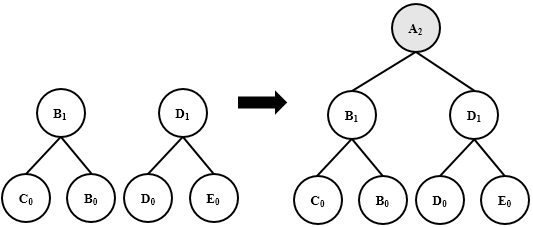
\includegraphics[width=6in]{images/increase-height.png}\\
		\caption{$A$ has $B_{1}, C_{1}$ in his forest and aggregates those two trees and creates $A_{2}$.}
		\label{fig:increase-height}
	\end{figure}\\
	It repeats the process until no two data-items in its forest have the same count value.
	An example of generating the payload by merging the data-items in the forest for the sensor node $A$ in Figure \ref{fig:at} is illustrated in the following example.
	% \ref{fig:commitment-tree-example-1}, \ref{fig:commitment-tree-example-2}, \ref{fig:commitment-tree-example-3}, \ref{fig:commitment-tree-example-4}.
			\begin{exmp} The commitment-payload generation process for node $A$ of Figure \ref{fig:at} is shown here.\\
				\begin{figure}[h!]
					\centering
					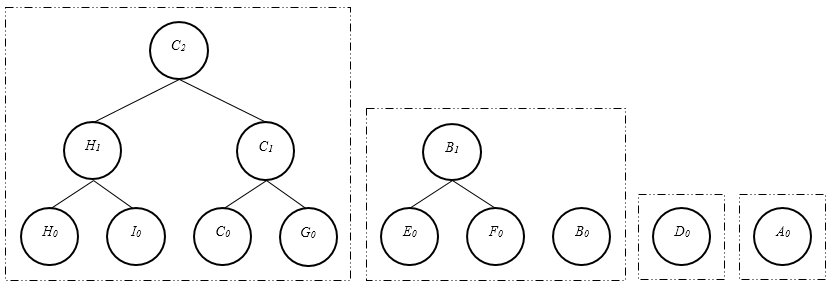
\includegraphics[width=6in]{images/commitment-tree-example-1.png}\\
					\caption{$A$ receives $C_{2}$ from $C$, $(B_{1},B_{0})$ from $B$, $D_{0}$ from $D$ and generates $A_{0}$. The commitment payload received from a given sensor node is indicated by dashed-line box.}
					\label{fig:commitment-tree-example-1}
				\end{figure}
				\begin{equation}
					\begin{array}{l}
						A_{0} = <A_{id}, 1, A_{value}, H(N||1||A_{value})>; \textsf{Sign}_{S_{A}}(A_{0}) \\
						D_{0} = <D_{id}, 1, D_{value}, H(N||1||D_{value})>; \textsf{Sign}_{S_{D}}(D_{0})\\
						B_{0} = <B_{id}, 1, B_{value}, H(N||1||B_{value})>; \textsf{Sign}_{S_{B}}(B_{0})\\
						B_{1} = <B_{id}, 2, B_{value}, H(N||2||B_{value}||E_{0}||F_{0})>; \textsf{Sign}_{S_{B}}(B_{1})\\
						\textcolor{red}{\textsf{Sign}_{S_{B}}(B_{0} || B_{1}), benefits}\\
						C_{2} = <C_{id}, 4, C_{value}, H(N||4||C_{value})||H_{1}||C_{1})>; \textsf{Sign}_{S_{C}}(C_{2})\\
						\end{array}
				\end{equation}

				\begin{figure}[h!]
					\centering
					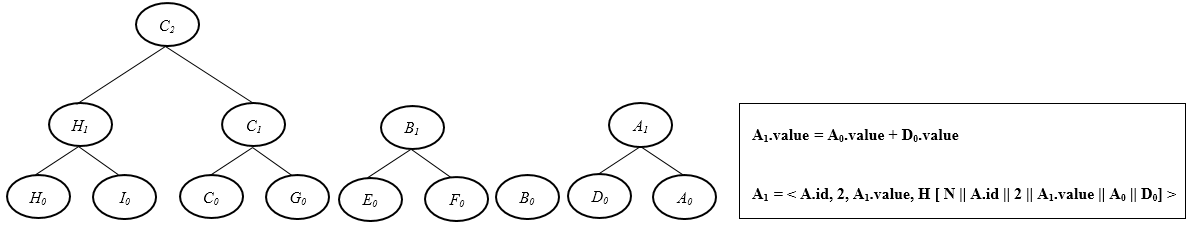
\includegraphics[width=6in]{images/commitment-tree-example-2.png}\\
					\caption{First Merge: $A_{1}$ vertex created by A.}
					\label{fig:commitment-tree-example-2}
				\end{figure}

				\begin{equation}
					\begin{array}{l}
				A_{1} = <A_{id}, 2, A_{1value}, H(N||2||A_{1value}||A_{0}||D_{0})>; \textsf{Sign}_{S_{A}}(A_{1})\\
				where\  A_{1value} = A_{value} + D_{value} \\
					\end{array}	
				\end{equation}
				\begin{figure}[h!]
					\centering
					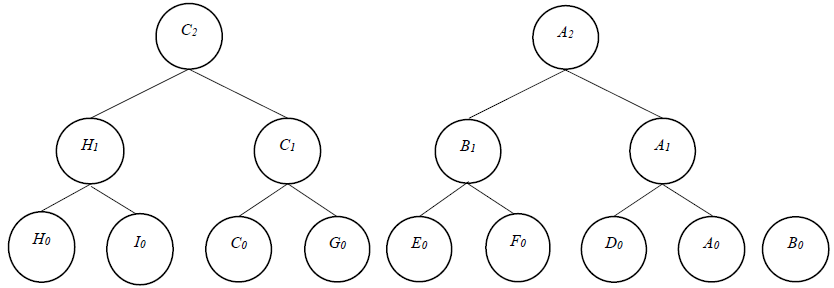
\includegraphics[width=\textwidth]{images/commitment-tree-example-3.png}\\
					\caption{Second Merge: $A_{2}$ vertex created by A.}
					\label{fig:commitment-tree-example-3}
				\end{figure}
				\begin{equation}
					\begin{array}{l}
						A_{2} = <A_{id}, 4, A_{2value}, H(N||4||A_{2value}||B_{1}||A_{1}) >; \textsf{Sign}_{S_{A}}(A_{2})\\
						where\  A_{2value} = B_{1value} + A_{1value} \\
					\end{array}
				\end{equation}
				\begin{figure}[h!]
					\centering
					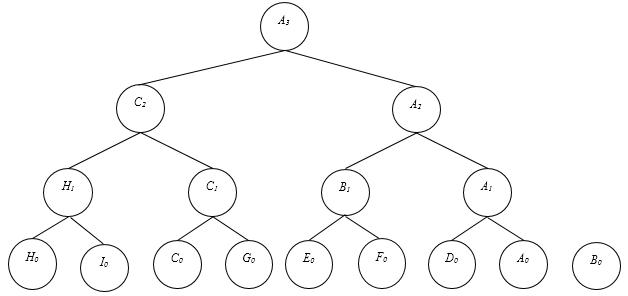
\includegraphics[width=6in]{images/commitment-tree-example-4.png}\\
					\caption{Third Merge: $A_{3}$ vertex created by A.}
					\label{fig:commitment-tree-example-4}
				\end{figure}
				\begin{equation}
					\begin{array}{l}
						A_{3} = <A_{id},8, A_{3value},H(N||8||A_{3value}||C_{2}||A_{2})>; \textsf{Sign}_{S_{A}}(A_{3})\\
						where\ A_{3value} = A_{2value} + C_{2value}
					\end{array}
				\end{equation}
			\end{exmp}
% chapter A Protocol for Commitment Tree Generation (end)

% Talk about the certificates:
	
% 	How many certificates does $A$ need to know in this example ?
% 	In the above example, $A$ need to know $D,B,C's$ certificate to verify their signatures.
% 	But if we use SHIA'a approach of creating commitment tree then $A$ need to know $E's$ certificate as well.
% 	Hence, being root in as many tree as possible is the more efficient.
\section{Bandwidth Analysis}
	For any given sensor node's forest with $n$ leaf vertices, has at most $\log n$ data-items in its payload.
	It has at most $(\log n) +1$ signatures in its payload.
	The highest possible count value is $\log n$, as all the trees are binary. 

	An intermediate sensor node $S$ with $\beta$ descendants in the aggregation tree, has at most $\log(\beta+1)$ data-items with their respective $\log(\beta+1)$ signatures in its payload.
	$S$ might need to send its payload signature $Sign(S_{p})$.
	At max, $S$ has to send a payload with $\log(\beta+1)$ data-items and $\log(\beta+1) +1$ signatures to its parent in the aggregation tree.
	
	Hence, sending signatures of the data-items causes $O(\log \beta)$ bandwidth overhead for each node in the network, where $\beta$ is the number of descendants of the sensor node. 
\section{Result checking}

\section{Performance Analysis}
	In addition to calculating its own data-items, all intermediate sensor nodes with $\beta$ descendants and $\zeta$ direct children need to do the following:
	\begin{itemize}
		\item To calculate and verify $O(\log \beta)$ signatures, creating $O(\log \beta)$ calculation overhead. 
		\item Needs sufficient memory to cache $O(\log \beta)$ certificates. 
		\item Needs enough memory to cache $\Omega(\zeta)$ certificates.
	\end{itemize}

	% Computation cost: Needs to calculate that many signatures. Needs to verify that many signatures.
	% Need to know that many certificates.

\section{Applications}
		The signature based aggregation scheme can be applied to do the \textbf{voting} in the network.
		And voting scheme can be used to solve many sensor network problems.
		For example, voting can be used to design the distributed algorithm for selecting a cluster head or node revocation system.
		In the voting scheme, following are the major security concerns: 
		\begin{itemize}
			\item The aggregate node needs to know that the vote is coming from the legit voter, no other voter is impersonating the vote of the legit voter.
			\item Only the intended aggregate node should be able to verify the vote.
			\item The aggregate node should not be able to tamper with the votes. 
			\item The aggregate node needs the proof that it aggregated the verified votes.
			\item The voter need the proof for which vote it sent to its aggregator.
		\end{itemize}
		For example, the base station wants to know the overall vote-count in the network.
		To do so, all the leaf nodes send their votes and the signature of their votes to their respective aggregate nodes in the network.
		The aggregate nodes receive votes with their signatures from all of their children voters.
		The aggregate nodes verify all the votes and count those votes.
		Then they forward the count and the signature of that count signed by the aggregate node to their respective parent in the aggregation tree.
		This process is repeated until the final count and its signature, is sent to the base station by the root of the aggregation tree.
				
\textbf{Node power level},
\textbf{Surveillance Application}
